\documentclass{article}
\usepackage[paperwidth=24cm,paperheight=12cm,margin=5mm]{geometry}
\usepackage{tikz}
\usepackage{amsmath}
\usetikzlibrary{arrows.meta,positioning,calc,backgrounds,fit}
\pagestyle{empty}
\definecolor{cpile}{RGB}{175,175,175}
\definecolor{csig}{RGB}{30,110,190}
\definecolor{cbad}{RGB}{200,40,40}
\definecolor{cgood}{RGB}{30,150,90}
\begin{document}
\noindent
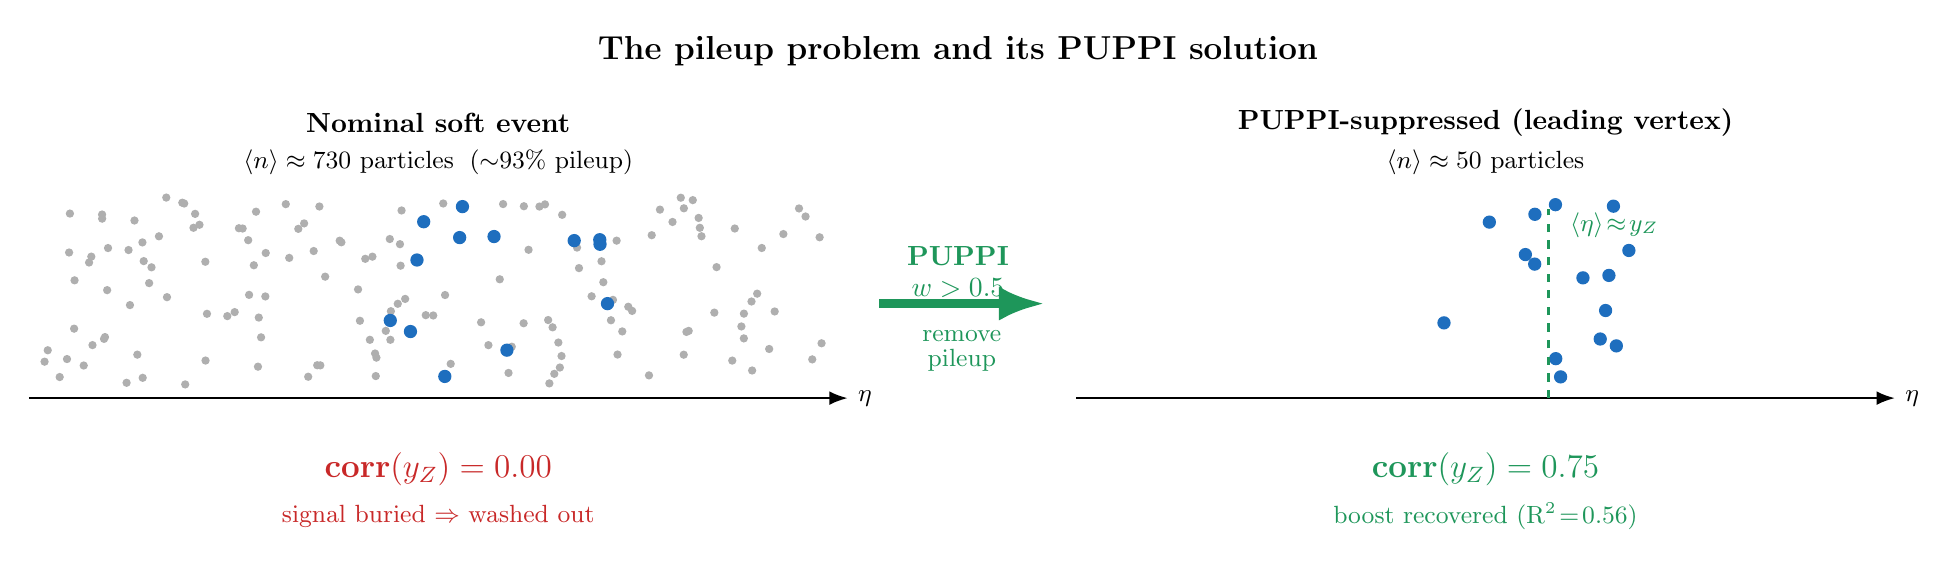
\begin{tikzpicture}[>=Latex,font=\sffamily]
\pgfmathsetseed{7}
% ===================== LEFT: nominal (pileup) =====================
\begin{scope}
  \draw[->,thick] (-5.2,0) -- (5.2,0) node[right,font=\small]{$\eta$};
  \node[font=\bfseries] at (0,3.5) {Nominal soft event};
  \node[font=\small,align=center] at (0,3.0) {$\langle n\rangle\approx730$ particles \;($\sim$93\% pileup)};
  % pileup dots (gray), uniform in eta, jittered in y
  \foreach \i in {1,...,150}{
    \pgfmathsetmacro\x{(rnd*10)-5}
    \pgfmathsetmacro\y{0.15+rnd*2.4}
    \fill[cpile] (\x,\y) circle (1.5pt);}
  % signal dots (blue), clustered near boost (+0.8)
  \foreach \i in {1,...,13}{
    \pgfmathsetmacro\x{0.8+(rnd-0.5)*3.2}
    \pgfmathsetmacro\y{0.2+rnd*2.3}
    \fill[csig] (\x,\y) circle (2.4pt);}
  \node[cbad,font=\bfseries\large] at (0,-0.9) {corr$(y_Z)=0.00$};
  \node[cbad,font=\small] at (0,-1.5) {signal buried $\Rightarrow$ washed out};
\end{scope}
% ===================== arrow =====================
\node[cgood,font=\bfseries,align=center] at (6.6,1.6) {PUPPI\\[-1pt]$w>0.5$};
\draw[->,line width=3pt,cgood] (5.6,1.2) -- (7.7,1.2);
\node[font=\small,cgood,align=center] at (6.65,0.6){remove\\[-2pt]pileup};
% ===================== RIGHT: PUPPI-suppressed =====================
\begin{scope}[xshift=13.3cm]
  \draw[->,thick] (-5.2,0) -- (5.2,0) node[right,font=\small]{$\eta$};
  \node[font=\bfseries] at (0,3.5) {PUPPI-suppressed (leading vertex)};
  \node[font=\small,align=center] at (0,3.0) {$\langle n\rangle\approx50$ particles};
  % only signal dots (blue), clustered near boost (+0.8) -> visible structure
  \foreach \i in {1,...,15}{
    \pgfmathsetmacro\x{0.8+(rnd-0.5)*3.4}
    \pgfmathsetmacro\y{0.25+rnd*2.3}
    \fill[csig] (\x,\y) circle (2.4pt);}
  % mean marker
  \draw[cgood,line width=1.3pt,dashed] (0.8,0) -- (0.8,2.4);
  \node[cgood,font=\small,right] at (0.95,2.2){$\langle\eta\rangle\!\approx\!y_Z$};
  \node[cgood,font=\bfseries\large] at (0,-0.9) {corr$(y_Z)=0.75$};
  \node[cgood,font=\small] at (0,-1.5) {boost recovered (R$^2\!=\!0.56$)};
\end{scope}
\node[font=\bfseries\large] at (6.6,4.4){The pileup problem and its PUPPI solution};
\end{tikzpicture}
\end{document}
